\documentclass{book}
%11pt,a4paper,twoside
\usepackage{polski}
\usepackage[utf8]{inputenc}
\usepackage[titletoc]{appendix}
\usepackage{tikz}
\usepackage{indentfirst}
\usepackage{comment}
\usepackage{hyperref}
 
\frenchspacing

%%%% TODO LIST GENERATOR %%%%%%%%%

%\usepackage{tikz}
\usepackage{manfnt}   % dangerous sign 
\usepackage{color}
\definecolor{brickred}      {cmyk}{0   , 0.89, 0.94, 0.28}

\makeatletter \newcommand \kslistofremarks{\section*{Uwagi} \@starttoc{rks}}
  \newcommand\l@uwagas[2]
    {\par\noindent \textbf{#2:} %\parbox{10cm}
{#1}\par} \makeatother


\newcommand{\ksremark}[1]{%
{\marginpar{\textdbend}{\color{brickred}{[#1]}}}%
\addcontentsline{rks}{uwagas}{\protect{#1}}%
}

%%%%%%%%%%%%%% END OF TODO LIST GENERATOR %%%%%%%%%%%


% ustawienia marginesow
%\usepackage[cm]{fullpage}
%\usepackage[top=2.5cm, bottom=2.5cm, inner=3.5cm, outer=2.5cm, twoside]{geometry}

% ustawienia obrazow %
\usepackage{graphicx}
\graphicspath{ {./assets/} }
\DeclareGraphicsExtensions{.pdf,.png,.jpg}

%ustawienia svg 
\usepackage{svg}
%\setsvg{inkscape=inkscape -z -D,svgpath=./assets/images/}

%nazwa aplikacji
\newcommand{\appName}{\emph{TravelGuide} }
%czy mogę zmienić nazwę aplikacji na "TravelGuide" zamiast "Wirtualny Przewodnik"? Czyli tak, jak jest logo, etc.?

% listing kodu
\usepackage{listings}
\usepackage{color}

\lstdefinelanguage{JavaScript}{
	keywords={typeof, new, true, false, catch, function, return, null, catch, switch, var, if, in, while, do, else, case, break},
	keywordstyle=\color{blue}\bfseries,
	ndkeywords={class, export, boolean, throw, implements, import, this},
	ndkeywordstyle=\color{darkgray}\bfseries,
	identifierstyle=\color{black},
	sensitive=false,
	comment=[l]{//},
	morecomment=[s]{/*}{*/},
	commentstyle=\color{purple}\ttfamily,
	stringstyle=\color{red}\ttfamily,
	morestring=[b]',
	morestring=[b]"
}

\lstset{
	language=JavaScript,
	extendedchars=true,
	basicstyle=\small\tt,
	showstringspaces=false,
	showspaces=false,
	numbers=left,
	numberstyle=\footnotesize,
	numbersep=9pt,
	tabsize=4,
	breaklines=true,
	showtabs=false,
	captionpos=b,
	belowskip=1.5em,
	aboveskip=1.5em
}

% document settings
\begin{document}	

\kslistofremarks

\cleardoublepage
%stara strona tytułowa
\begin{comment}
	\begin{titlepage}
		\begin{center}
			
\includegraphics[width=4cm]{assets/images/polsl.jpg}\\[1cm]
			\textsc{\LARGE{Politechnika Śląska}}\\[0.5cm]
			\textsc{\LARGE{Wydział Automatyki, Elektroniki i~Informatyki}}\\[0.5cm]
			\textsc{\LARGE{Kierunek Informatyka}}\\[2.5cm]
			\LARGE{Projekt inżynierski}\\[1cm]
			\begingroup
			\fontsize{14pt}{17pt}\selectfont
		Wirtualny przewodnik dla urządzeń mobilnych
			\endgroup
		\end{center}
		\vspace{5cm}
		\begingroup
		\fontsize{14pt}{17pt}\selectfont
		\textbf{Autor:} Katarzyna Biernat\\
		\textbf{Kierujący pracą:} dr inż. Krzysztof Simiński\\
		\endgroup
		
		\vspace{3.5cm}
		\begingroup
		\fontsize{12pt}{14pt}\selectfont
		\begin{center}
			Gliwice, styczeń 2015
		\end{center}
		\endgroup
	\end{titlepage}
\end{comment}

%%%%%%%%   front.tex


% *************** Strona tytu³owa ***************
\pagestyle{empty}
\sffamily

\noindent
\begin{center}
    \Large
    Politechnika Śląska\\
    Wydział Automatyki, Elektroniki i Informatyki
    %\\ Nazwa kierunku
\end{center}

\begin{figure}[h]
\begin{center}

\includegraphics[width=0.2\textwidth]{images/polsl.pdf}
\end{center}
\end{figure}

\vfill\vfill
\begin{center}
    \Large
    Katarzyna Biernat
\end{center}

\vfill
\begin{center}
    \Huge\bfseries
    Wirtualny przewodnik dla urządzeń mobilnych
\end{center}

\vfill
\begin{center}
    \Large
    projekt inżynierski
\end{center}

\vfill\vfill\vfill
\begin{center}
    \Large
    Promotor/kierujący pracą: dr inż. Krzysztof Simiński
\end{center}

\vfill
\begin{center}
\large
   Gliwice, \today
\end{center}

\cleardoublepage

%% *************** Dedykacja ***************
%\vspace*{\fill}
%{\hfill\sffamily\itshape Pracę dedykuję \ldots}
%\cleardoublepage

\rmfamily
\normalfont

% *************** Spis treœci ***************
\pagenumbering{Roman}
\pagestyle{headings}
\tableofcontents

% *************** Koniec front matter ***************


%%%%%%%%  end of front

	
\mainmatter % powoduje, ze wlasciwa czesc pracy ma strony numerowe od 1 cyframi arabskimi
	
	\chapter{Wstęp}
		\section{Temat}
	
		\section{Cel}
		Celem niniejszego projektu jest stworzenie przyjaznej platformy dedykowanej dla osób podróżujących. Program ma ułatwić użytkownikowi zwiedzanie nowych miejsc oraz zupełnie zastąpić tradycyjny, książkowy przewodnik. Na całość składa się aplikacja mobilna na platformę Windows Phone 8.1 oraz aplikacja działająca w przeglądarce internetowej. 

		\section{Motywacja}
	
		\begin{figure}		
			\centering
			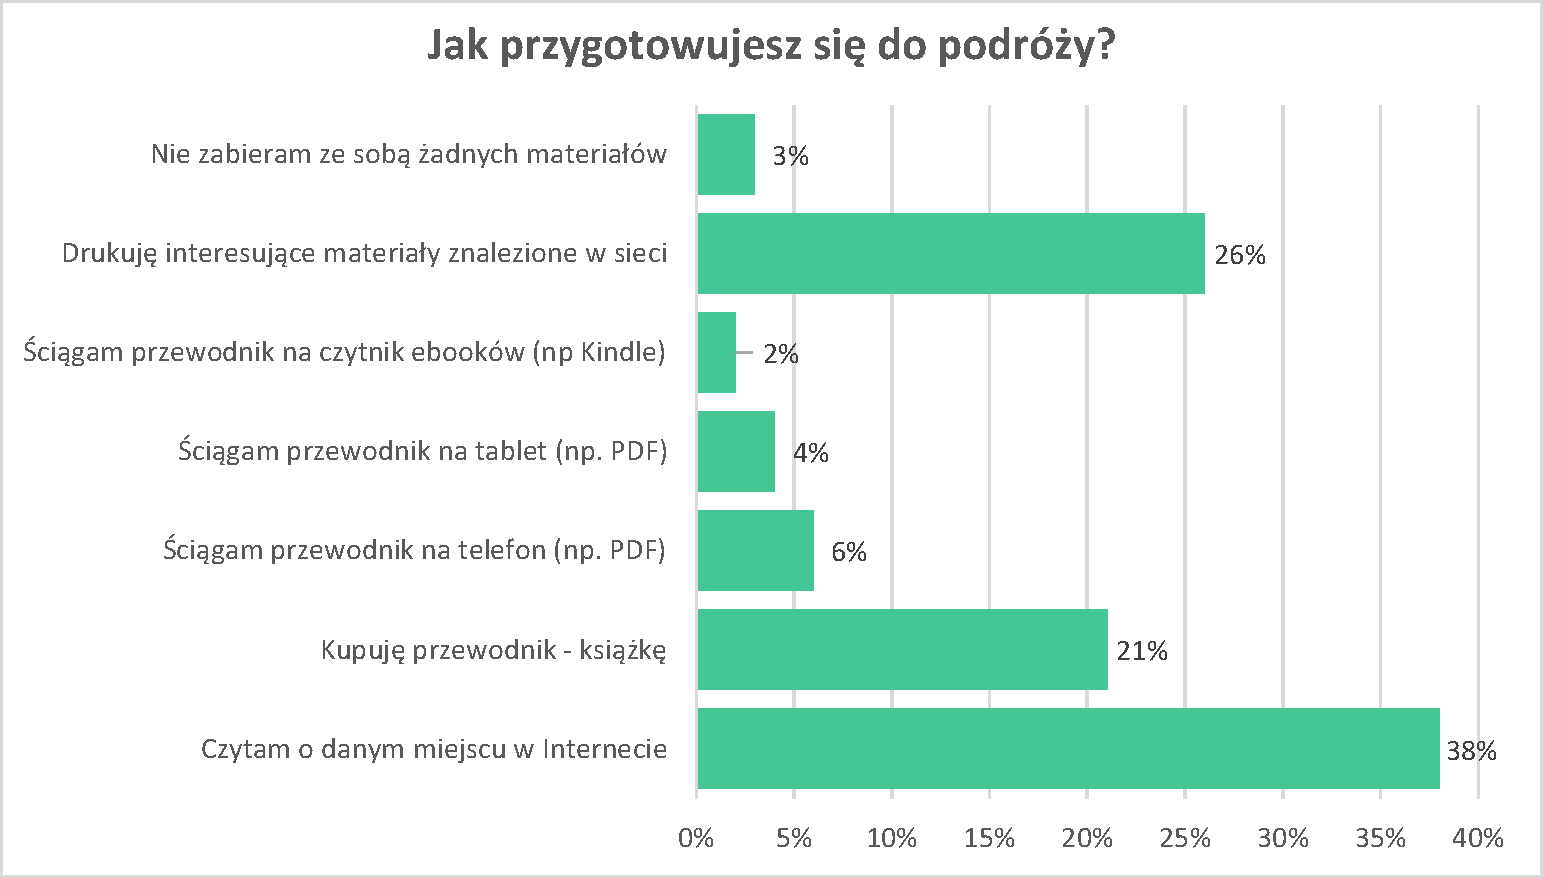
\includegraphics[width=1.0\textwidth]{images/fly4freeAnkieta.pdf}
			\caption{Wyniki ankiety przeprowadzonej wśród użytkowników forum fly4free.pl}
			\label{fig:fly4freeAnkieta}
		\end{figure}
		% nie umiem zrobić, żeby font był taki jak w reszcie dokumentu :( pdf_tex mnie nie słucha :(
	
		Obecnie na rynku istnieje nisza, jeśli chodzi o tego typu rozwiązania. W Internecie można znaleźć bardzo wiele różnych informacji o ciekawych miejscach turystycznych, brakuje jednak przyjaznej formy przedstawienia ich podróżnikowi. 
		
		Rysunek~\ref{fig:fly4freeAnkieta} przedstawia wyniki ankiety przeprowadzonej wśród 234 użytkowników forum Fly4Free.pl \cite{id:fly4free}. Jak się okazuje, zdecydowana większość podróżników zakupuje przewodnik o miejscu docelowym bądź pobiera stosowne informacje z sieci i drukuje je na swój użytek.
		
		Aplikacja \appName ma na celu połączenie zalet obu tych rozwiązań. Reprezentuje informacje w podobny sposób jak tradycyjny, książkowy przewodnik przy jednoczesnej możliwości szybkiej aktualizacji informacji. Ponadto dzięki temu, że zawiera się w smartfonie podróżnika, zwalnia go z noszenia ciężkich książek lub nieporęcznych drukowanych kartek. 
			
		Dzięki wykorzystaniu nowoczesnych technologii, aplikacja może podawać użytkownikowi najciekawsze informacje bazując na jego danych geolokalizacyjnych. 
	
	
	\chapter{Wprowadzenie do problemu}
	%Co tu powinno się znaleźć?
	\ksremark{Na razie proszę się tym nie przejmować. Zajmiemy się tym, gdy będzie więcej treści.}
	
	\chapter{Technologia}
		\section{Narzędzia}		
			\subsection{Środowisko programistyczne}
				
			Całość projektu została zrealizowana za pomocą Visual Studio 2013. Jest to jedno z popularniejszych środowisk programistycznych, wyprodukowane przez firmę Microsoft. Mimo że nie jest to środowisko bezpłatne, projekt mógł zostać zrealizowany bez ponoszenia kosztów dzięki licencji akademickiej \textit{DreamSpark}. 
			
			Visual Studio 2013 w pełni wspiera rozwijanie oprogramowania w platformie .NET; zarówno rozwiązania mobilne jak i internetowe. Poza tym, dzięki szeregowi dostępnych bibliotek, wspomaga pracę z HTML, LESS oraz JavaScript.
			
			Środowisko to zostało wybrane ze względu na następujące zalety:
			\begin{itemize}
				\item bardzo  dobra obsługa \textit{IntelliSense} dla języka C\#;
				\item wiele pomocnych rozszerzeń, np. \textit{Web Essentials};
				\item wsparcie dla składni języków HTML\footnote{\emph{HyperText Markup Language} -- hipertekstowy język znaczników wykorzystywany do tworzenia stron internetowych.}, CSS\footnote{\emph{Cascading Style Sheets} -- kaskadowe arkusze stylów służące do opisu formy prezentacji strony WWW.} i JavaScript;
				\item wbudowany emulator Windows Phone;
				\item gotowe szablony, które przyspieszają pracę z projektem.
			\end{itemize}
			
			\subsection{System kontroli wersji}
			
			Pomimo że projekt realizowany był indywidualnie, zdecydowano się na wykorzystanie systemu kontroli wersji. Na rynku dostępnych jest wiele takich systemów. Do najpopularniejszych należą: GIT \cite{id:GIT}, Mercurial \cite{id:Mecurial}, SVN \cite{id:SVN}, Bazaar \cite{id:Bazaar} oraz TFS \cite{id:TFS}.
			Podczas projektu zdecydowano się na wykorzystanie systemu GIT. Został on wybrany z wielu powodów. Jest to system rozproszony, więc jego repozytoria są relatywnie małe (np. w porównaniu do SVN). Ponadto GIT oferuje wiele funkcjonalności, które ułatwiają pracę z projektem, m.in. tzw. gałęzie \ksremark{SVN też umożliwia rozgałęzianie}, etykiety czy lokalną przestrzeń roboczą. Nie bez znaczenia był także fakt, że autorka ma doświadczenie z tym systemem kontroli wersji.

			Repozytorium zostało umieszczone w serwisie Github.com\footnote{Serwis dostępny pod adresem \url{http://github.com}}, który agreguje projekty z całego świata. Portal oferuje przejrzysty interfejs oraz możliwość graficznego przeglądania historii projektu.
		
		\section{Technologia wykorzystana w części serwerowej}
		
		Część serwerowa, realizowana jako WebService, wykonana została z wykorzystaniem platformy ASP.NET WebApi 2 \cite{id:WebApi}. Całość opiera się na platformie .NET 4.5 i napisana jest w języku C\#.
		
		W tej części wykorzystano szereg bibliotek. Aby przyspieszyć pracę i zapewnić większe bezpieczeństwo aplikacji, do celów identyfikacji i uwierzytelniania użytkowników została wykorzystana biblioteka AspNet.Identity \cite{id:ASPIdentity}.
		
		Do pracy z kolekcjami wykorzystano bibliotekę LINQ. Jest to zestaw niezwykle przydatnych narzędzi, które ułatwiają pracę z takimi strukturami jak listy, kolejki i inne implementujące interfejs \texttt{IEnumerable}.
		
		Nieodzowna okazała się być biblioteka Newtonsoft.Json \cite{id:NewtonsoftJSON}, która wspomaga formatowanie obiektów na kod JSON\footnote{\emph{JavaScript Object Notation} -- tekstowy format wymiany danych}. Wszystkie akcje zwracające dane zwracają je właśnie w tym formacie. Komunikat w formacie JSON jest literałem obiektu języka JavaScript. Dane przekazywane są jako tablica asocjacyjna a wszystkie dane są zmiennymi.
		
		Jako że WebService działa w innej domenie niż aplikacja użytkownika, niezbędne było dodanie odpowiednich nagłówków HTTP, aby umożliwić zapytania z innej domeny (\emph{Cross Origin Requests}). Bardzo ułatwia to biblioteka Microsoft.AspNet.Cors \cite{id:ASPCors}. Dodaje ona szereg nagłówków wraz z odpowiednio dobranymi parametrami.
		
		WebService komunikuje się z bazą danych, która działa w oparciu o silnik SQL Server 2014 \cite{id:SQLServer}. Komunikacja odbywa się z wykorzystaniem biblioteki Entity Framework \cite{id:EntityFramework}. Jest to biblioteka typu ORM\footnote{\emph{Object-Relational Mapping} -- mapowanie obiektowo-relacyjne. },
		która umożliwia mapowanie wyników pobranych z bazy danych na wcześniej przygotowane modele. Modele te są następnie mapowane na modele przejściowe (\emph{ViewModels}) za pomocą biblioteki AutoMapper \cite{id:Automapper}.
		
		\section{Technologia wykorzystana w części internetowej} 
			
		Aplikacja internetowa napisana została w modelu \emph{client-side}. Oznacza to, że cała aplikacja interpretowana jest po stronie przeglądarki i nie wymaga specjalistycznego serwera. Aby działała poprawnie, wystarczy dowolny serwer HTTP. Kod został napisany przy użyciu następujących języków: Javascript, HTML i LESS\footnote{\emph{Leaner CSS} -- dynamiczny język arkuszy stylów.}. 
        %		
		Aplikacja stworzona jest w oparciu o platformę AngularJS \cite{keylist}. Jest to zestaw otwartych bibliotek języka JavaScript wspierany przez firmę Google. Umożliwia tworzenie aplikacji internetowych, z których można korzystać bez przeładowania strony (\emph{Single Page Application}). Dane ładowane są w tle dzięki asynchronicznym zapytaniom do WebService realizowanym przez JavaScript.
		
		Zostały również zastosowane poboczne biblioteki. Do najważniejszych zależą:
		
		\begin{description}
			
			\item[LeafletJS] \cite{id:Leaflet} -- 
			umożliwia sprawne dodawanie map do strony. Do wyświetlania map wybrany został silnik OpenStreetMap \cite{id:OpenStreetMaps} ze względu na swoją otwartą licencję.
			\item[jQuery] \cite{id:jQuery} -- 
			jest to zestaw bibliotek pomocniczych dla języka JavaScript. Rozszerza funkcjonalność i upraszcza składnię. W prostszy sposób pozwala na dostęp i manipulację elementami DOM.
			\item[Bootstrap] \cite{id:Bootstrap} -- 
			zestaw bibliotek, który dołączony jest do Twitter Bootstrap. Dostarcza takie moduły jak np. interaktywne wyskakujące okna, animacje zamknięcie i in.
			\item[AngularTranslate.js] \cite{id:AngularTranslate} -- 
			biblioteka rozszerzająca możliwości platformy Angular o implementację wielojęzyczności.  
		
		\end{description}
				
		Za część graficzną aplikacji odpowiada zmodyfikowany przez autorkę szablon AdminLTE \cite{id:AdminLTE} napisany w oparciu o Twitter Bootstrap. Szablon opisany jest językiem LESS, który jest następnie transformowany do CSS.
		
		\section{Technologia wykorzystana w części mobilnej}
	
		Na część mobilną składa się aplikacja dedykowana dla platformy Windows Phone 8.1. Projekt zrealizowany został w modelu Universal Apps, więc cała logika wydzielona jest do osobnego projektu.
		
		Aplikacja wykonana została przy wykorzystaniu platformy .NET, języka C\# oraz XAML. Zaimplementowany został wzorzec architektoniczny MVVM (\emph{Model View ViewModel}, \emph{vide} rozdział \ref{sec:ArchitekturaAplikacjiMobilnej}). W tym celu do projektu dołączona została biblioteka MVVM Light \cite{id:MVVMLight}. 
		
		Aplikacja pobiera dane z WebService i zapisuje je w swojej lokalnej bazie danych. Działa ona dzięki SQLight \cite{id:SQLite}. Do projektu dołączony jest adapter SQLite. Pobrane dane parsowane są do obiektów za pomocą biblioteki Newtonsoft.JSON.

	\chapter{Specyfikacja wewnętrzna}
		\section{Architektura}
		
		\begin{figure}		
			\centering
			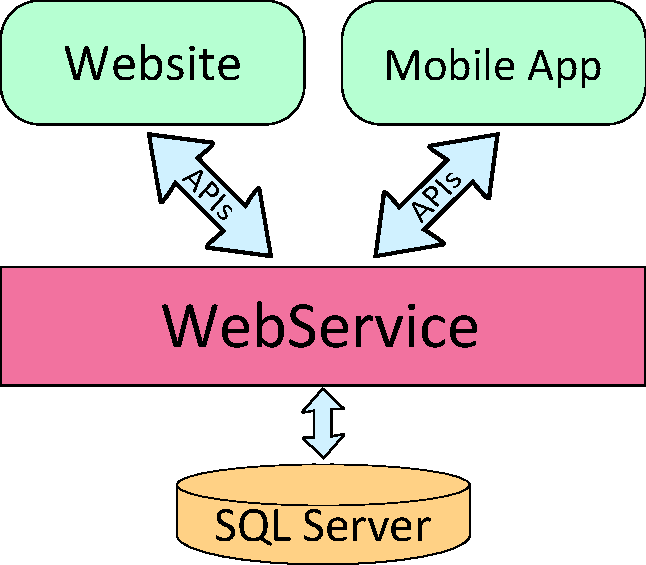
\includegraphics[width=0.5\textwidth]{images/architektura.pdf}
			\caption{Architektura systemu}
			\label{fig:architektura}
		\end{figure}
		
		Na cały system składają się trzy aplikacje: aplikacja mobilna (\emph{Mobile app}), aplikacja internetowa (\emph{Website}) oraz aplikacja serwerowa (\emph{WebService}). Związek pomiędzy tymi aplikacjami przedstawiony jest na rysunku \ref{fig:architektura}. 
			
			\subsection{Architektura aplikacji serwerowej}
			
			\begin{figure}
				\centering
				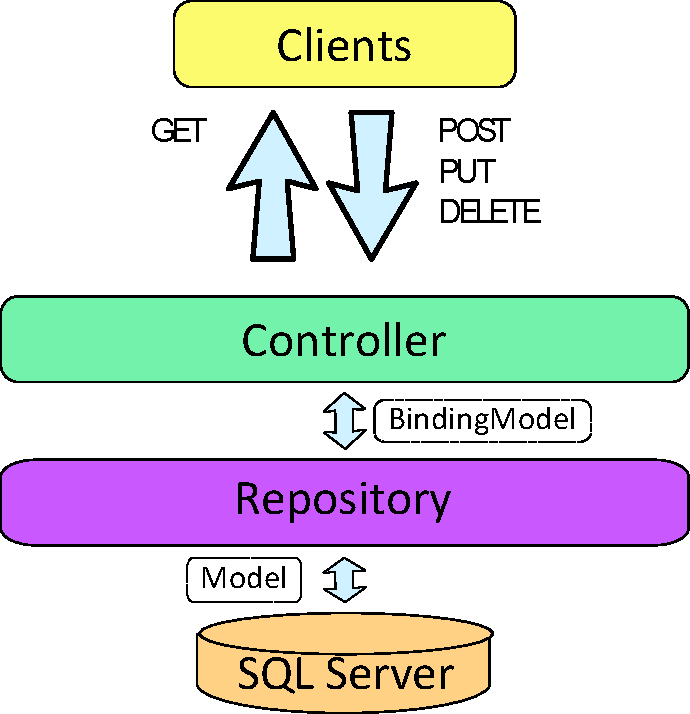
\includegraphics[width=1\textwidth]{images/architektura_server.pdf}
				\caption{Architektura aplikacji serwerowej}
				\label{fig:architektura_server}
			\end{figure}
			
			Aplikacja serwerowa stworzona jest przy wykorzystaniu platformy ASP.NET WebApi 2 i zgodnie ze wzorcem architektonicznym REST\footnote{\emph{Representational State Transfer}}. Wzorzec ten zakłada kilka warunków:
			
			\begin{description}
				
				\item[Klient-serwer] -- aplikacja powinna składać się z~dwóch odrębnych części: klienta i serwera. Klient nie powinien mieć dostępu do magazynu danych. Serwer z kolei nie powinien zawierać informacji na temat interfejsu użytkownika. I tak też aplikacja serwerowa systemu \appName jest jedyną, która ma dostęp do bazy danych. Nie zawiera ona żadnych widoków, a ze światem 				komunikuje się za pomocą zapytań HTTP\footnote{\emph{Hypertext Transfer Protocol} – protokół przesyłania dokumentów hipertekstowych}.
				\item[Bezstanowość] -- każde żądanie HTTP (\emph{request}) wysyłane do serwera jest niezależne od pozostałych. I tak też w aplikacji serwerowej systemu \appName, za odbiór żądań odpowiada warstwa kontrolera. Każda akcja kontrolera obsługuje jedno żądanie. Akcje są od siebie niezależne.
				\item[Wielowarstwowość] -- klient nie wie, czy jest podłączony bezpośrednio do serwera, czy też otrzymuje informacje przez systemy pośrednie. Dzięki takiej skalowalności, systemy pośrednie mogą zostać wykorzystane, aby zwiększyć wydajność całości. Aplikacja serwerowa systemu \appName przyjmuje żądania HTTP a odpowiedź wysyła w formacie JSON. Można więc dołożyć kolejne systemu pośrednie zgodnie z zapotrzebowaniem. 
				\item[Cache'owalność] -- \ksremark{to jakoś trzeba będzie napisać po polsku} %jak to przetłumaczyć? :(
				serwer powinien zwracać informację, które z odpowiedzi mogą zostać zapisane w pamięci podręcznej cache przeglądarki. W przypadku aplikacji serwerowej systemu \appName nie jest to zaimplementowane, gdyż żadna z odpowiedzi nie powinna być zapisywana.
				
			\end{description}
			
			Wewnętrznie aplikacja składa się z wielu warstw, które komunikują się ze sobą. Każde odebrane zapytanie HTTP jest obsługiwane przez odpowiednią akcję kontrolera. Zapytania realizowane są czterema standardowymi metodami HTTP: \emph{GET}, \emph{POST}, \emph{PUT}, \emph{DELETE}.
			
			Zazwyczaj akcja wymaga interakcji z bazą danych. Kontroler nie komunikuje się z nią jednak bezpośrednio. Zamiast tego składa odpowiednio sparametryzowane zapytanie do warstwy repozytorium. Parametrem może być cyfra (\texttt{Integer}), ciąg znaków (\texttt{String}) lub obiekt typu modelu wiążącego (\emph{Binding Model}). Parametr może być także pusty. 
			
			Repozytorium przetwarza żądanie. Jeżeli parametrem był obiekt typu modelu wiążącego mapuje go na model, a następnie za pomocą \emph{Entity Framework} komunikuje się z bazą danych. Rezultat jest następnie ponownie mapowany na model wiążący i przekazywany do akcji kontrolera. Kontroler zwraca wynik w postaci odpowiedzi HTTP (\emph{HTTP Response}).
			
			Schemat architektury aplikacji mobilnej przedstawiony jest na rysunku \ref{fig:architektura_server}. 			
			
			\subsection{Architektura aplikacji internetowej}		
			
			\begin{figure}
				\centering
				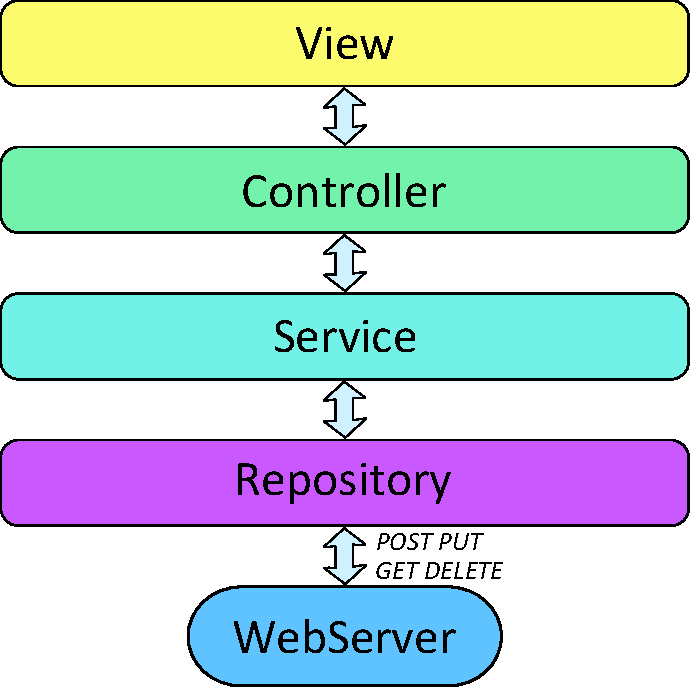
\includegraphics[width=1\textwidth]{images/architektura_webapp.pdf}
				\caption{Architektura aplikacji internetowej}
				\label{fig:architektura_webapp}
			\end{figure}

			Aplikacja internetowa została stworzona przy użyciu platformy AngularJS i~w~całości działa bez przeładowania strony (\emph{Single Page Application}). Zawiera główny widok napisany w języku HTML, do którego w zależności od kontekstu załączane są widoki cząstkowe (\emph{partial views}). Z każdym widokiem powiązany jest kontroler. 
			
			Kiedy użytkownik wchodzi w interakcję z aplikacją, jego akcje są wysyłane do odpowiednich akcji kontrolera. Kontroler następnie obsługuje daną operację lub, jeżeli jest ona bardziej skomplikowana, odwołuje się do odpowiedniej metody z warstwy serwisu. Jeżeli wymagane jest pobranie danych z WebService, warstwa serwisu komunikuje się z warstwą repozytorium, która następnie wysyła odpowiednio skonstruowane zapytanie. Otrzymany wynik jest przekazywany z~powrotem do warstwy serwisu, przetwarzany, przekazywany do kontrolera i~wiązany (\emph{Bind}) z~widokiem.								

			Schemat architektury aplikacji mobilnej przedstawiony jest na rysunku \ref{fig:architektura_webapp}.			
			
			\subsection{Architektura aplikacji mobilnej}
			\label{sec:ArchitekturaAplikacjiMobilnej}	
			
			\begin{figure}
				\centering
				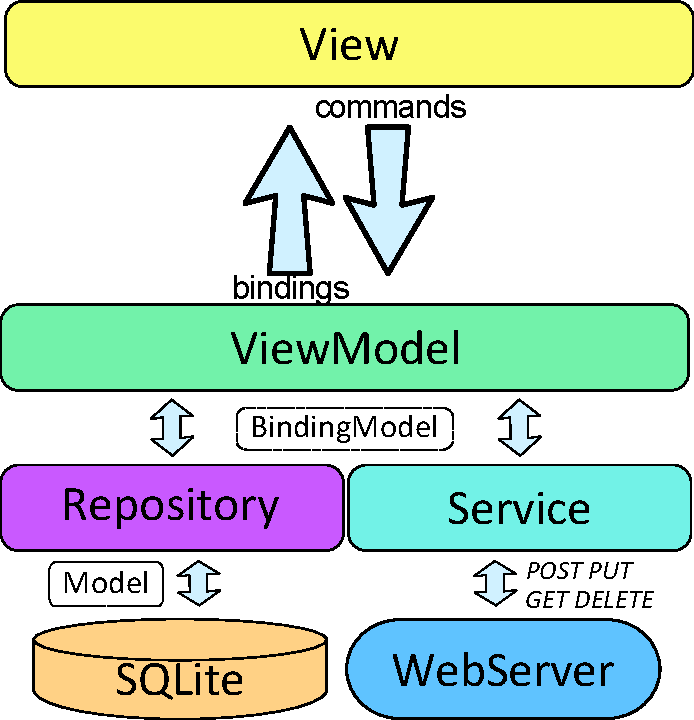
\includegraphics[width=1\textwidth]{images/architektura_mobile.pdf}
				\caption{Architektura aplikacji mobilnej}
				\label{fig:architektura_mobile}
			\end{figure}
			
			Aplikacja mobilna dedykowana jest dla platformy Windows Phone 8.1. Została stworzona przy użyciu wzorca MVVM (\emph{Model View ViewModel}). Wzorzec ten polega na rozdzieleniu warstwy widoku (\emph{View}) od warstwy danych (\emph{Model}). Są one połączone za pomocą warstwy pośredniej (\emph{ViewModel}), która zawiera większą część logiki związanej z prezentacją danych. \ksremark{Tu przydałby się rysunek modelu MVVM.}
			
			Program przy pierwszym uruchomieniu łączy się z aplikacją serwerową i~pobiera dane, do których uprawniony jest zalogowany użytkownik. Dane te są zapisywane w lokalnej bazie danych obsługiwanej przez silnik SQLite. 
			
			Użytkownik wchodzi w interakcję z aplikacją przy pomocy zachowań typowych dla obsługi aplikacji mobilnych. Są to gesty takie jak dotknięcie ekranu, dłuższe przytrzymanie ekranu czy posuwisty ruch dłonią po ekranie smartfona. 
			Po stronie aplikacji odbiorcą takich poleceń jest warstwa widoku (\emph{View}). Komunikuje się ona następnie z warstwą pośrednią (\emph{ViewModel}) wprost lub za pomocą konwerterów (\emph{Converter}). Komunikacja odbywa się dzięki wykorzystaniu poleceń (\emph{Commands}. 
			
			Warstwa pośrednia realizuje zadanie zadane przez użytkownika. Jeżeli wymaga to komunikacji z bazą danych, łączy się ona z warstwą repozytorium (\emph{Repository}). Repozytorium operuje na dwóch typach obiektów: na modelach (\emph{Model}) i na modelach wiążących (\emph{Binding model}). Modele odwzorowują schemat bazy danych w postaci obiektów języka C\# i są wykorzystywane w komunikacji z nią. Modele wiążące to modele zmodyfikowane na potrzeby danego zadania.  % \ksremark{To zdanie jest trochę niejasne, warto by je nieco rozwinąć.}
			Są one zmodyfikowane o dodatkowe pola, zbędne pola nie są zaś uwzględnione. Przykładowo, model wiążący wykorzystywany do rejestracji użytkownika stworzony jest na bazie modelu użytkownika. Nie uwzględnia on takich informacji jak "Data rejestracji" bądź "Konto Aktywne". Z drugiej strony jest uzupełniony o takie pole jak "Powtórz hasło".
			
			Za komunikację z aplikacją serwerową odpowiada warstwa serwisów (\emph{Service}), która wysyła do niej odpowiednie zapytania w formacie RESTful. 
			
			Warstwa pośrednia nie wie o istnieniu modeli. Od repozytorium otrzymuje ona jedynie kolekcje modeli wiążących. Finalnie są one przetwarzane i przekazywane do warstwy widoku za pomocą mechanizmu wiązania (\emph{binding}).
			
			Schemat architektury aplikacji mobilnej przedstawiony jest na rysunku \ref{fig:architektura_mobile}. 
			
		
		\section{Najważniejsze algorytmy}
		\section{Przypadki użycia}
		
		
	\chapter{Specyfikacja zewnętrzna}
		\section{Instrukcja obsługi}
		\section{Wymagania}
		
		Aplikacja mobilna zaprojektowana jest z myślą o platformie \emph{Windows Phone 8.1}. Na chwilę obecną nie jest dostępna dla użytkowników systemów \emph{Android} czy \emph{iOS}, jednakże docelowo zostanie dodane wsparcie dla tych platform. Jeżeli użytkownik posiada telefon z systemem \emph{Windows Phone 8}, powinien najpierw zaktualizować swój system. Następnie może pobrać i korzystać z aplikacji. System \emph{Windows Phone 7} nie jest wspierany.
		
		Aplikacja internetowa do poprawnego działania wymaga nowoczesnej przeglądarki z włączoną obsługą JavaScript. Wspierane przeglądarki:
		\begin{itemize}
			\item Google Chrome w wersji 39 lub nowszy;
			\item Mozilla Firefox w wersji 32 lub nowszy;
			\item Opera w wersji 26 lub nowsza;
			\item Internet Explorer 11 lub nowszy.
		\end{itemize}
		
		Aplikacja internetowa działa także na urządzeniach o mniejszych rozdzielczościach takich jak tablety czy telefony.
		
		\section{Instalacja}
		
		Aplikacja mobilna \appName w chwili obecnej zainstalowana może być jedynie na telefonach z odblokowaną opcją deweloperską. Docelowo jednak program zostanie umieszczony w sklepie \emph{Windows Store}, skąd będzie dostępny do pobrania dla użytkowników polsko- i angielskojęzycznych. 
		
		Aplikacja internetowa nie wymaga instalacji. Dostępna jest dla każdego, kto jest podłączony do Internetu, dysponuje kompatybilną przeglądarką internetową i posiada uprawnienia do dodawania nowych przewodników. 
		
	\chapter{Testowanie}
	
	\chapter{Wnioski końcowe}
	
	\chapter{Zakończenie}
	
	
	\bibliographystyle{plain}
	\bibliography{bibliografia}
	
\end{document}

